\section{Multiscale Representation and the Fourier Viewpoint}

Section 3.2 emphasized the spatial side of convolution:
it is local,
it shares weights across position,
and it builds larger receptive fields by composition.
That viewpoint is indispensable, but it is not the whole story.
Convolution also belongs to a classical mathematical tradition in signal processing and harmonic analysis.
The same operator that acts locally in the spatial domain acts diagonally in the Fourier domain.
This second viewpoint helps explain what convolutional filters do,
why some filters smooth while others sharpen or detect edges,
and why stacked convolutional layers may be interpreted as multiscale operators rather than merely as engineering devices.

\medskip

The central thesis of this section is that convolutional networks should be understood simultaneously in two linked ways.
In the spatial domain, a filter detects local configurations by sliding over the input.
In the frequency domain, the same filter amplifies some Fourier modes and suppresses others.
A mathematically mature understanding of convolution comes from holding both pictures at once.

\subsection*{Discrete Fourier transform, filtering, and frequency response}

We begin with the finite-dimensional setting, where everything can be written explicitly.
Because the cleanest algebra is obtained under circular boundary conditions, we state the main theorem for circular convolution.
This is not a practical limitation.
It isolates the core principle that Fourier analysis diagonalizes translation-invariant linear operators.

\begin{definition}[Discrete Fourier transform]
Let $x=(x_0,\dots,x_{N-1}) \in \mathbb{C}^N$ and let
\[
\omega_N = e^{-2\pi i/N}.
\]
The \emph{discrete Fourier transform} (DFT) of $x$ is the vector $\widehat{x} \in \mathbb{C}^N$ with entries
\[
\widehat{x}_k = \sum_{n=0}^{N-1} x_n\, \omega_N^{kn},
\qquad k=0,\dots,N-1.
\]
The inverse transform is given by
\[
 x_n = \frac{1}{N}\sum_{k=0}^{N-1} \widehat{x}_k\, \omega_N^{-kn},
 \qquad n=0,\dots,N-1.
\]
\end{definition}

\begin{definition}[Circular convolution]
Let $x,w \in \mathbb{C}^N$.
Their \emph{circular convolution} is the vector $y = w \circledast x \in \mathbb{C}^N$ defined by
\[
 y_n = (w \circledast x)_n = \sum_{m=0}^{N-1} w_m\, x_{(n-m) \bmod N},
 \qquad n=0,\dots,N-1.
\]
\end{definition}

\begin{definition}[Filtering and frequency response]
A \emph{filter} is a linear operator that transforms a signal into another signal, typically by emphasizing some patterns and suppressing others.
When the filter is given by convolution with a kernel $w$, its \emph{frequency response} is the Fourier transform $\widehat{w}$.
The magnitude $|\widehat{w}_k|$ tells how strongly the filter passes or attenuates the $k$th Fourier mode, while the phase of $\widehat{w}_k$ determines how that mode is shifted.
\end{definition}

\medskip

These definitions already suggest why Fourier analysis is useful.
A signal may be complicated when viewed as a list of spatial values, but much simpler when decomposed into oscillatory components.
A convolutional kernel may look like a short local stencil in space, yet in frequency it becomes a mode selector.
Low-pass filters preserve slowly varying components.
High-pass filters emphasize rapid variation.
Band-pass filters isolate intermediate ranges.

\subsection*{The discrete convolution theorem}

The key result is the finite-dimensional convolution theorem.
It is one of the most important identities linking deep learning to classical signal processing.

\begin{theorem}[Discrete convolution theorem]
Let $x,w \in \mathbb{C}^N$, and let $\widehat{x}$ and $\widehat{w}$ denote their discrete Fourier transforms.
Then the DFT of their circular convolution satisfies
\[
 \widehat{w \circledast x}_k = \widehat{w}_k \, \widehat{x}_k,
 \qquad k=0,\dots,N-1.
\]
Equivalently,
\[
 \mathcal{F}(w \circledast x) = \mathcal{F}(w) \odot \mathcal{F}(x),
\]
where $\odot$ denotes pointwise multiplication.
\end{theorem}

\begin{proof}
Fix $k$.
By definition,
\[
\widehat{w \circledast x}_k
= \sum_{n=0}^{N-1} (w \circledast x)_n\, \omega_N^{kn}
= \sum_{n=0}^{N-1}\sum_{m=0}^{N-1} w_m\, x_{(n-m)\bmod N}\, \omega_N^{kn}.
\]
Interchange the order of summation:
\[
\widehat{w \circledast x}_k
= \sum_{m=0}^{N-1} w_m \sum_{n=0}^{N-1} x_{(n-m)\bmod N}\, \omega_N^{kn}.
\]
Now make the change of variables $r=(n-m) \bmod N$.
Then $n \equiv r+m \pmod N$, and because the summation runs over a complete residue system, we obtain
\[
\sum_{n=0}^{N-1} x_{(n-m)\bmod N}\, \omega_N^{kn}
= \sum_{r=0}^{N-1} x_r\, \omega_N^{k(r+m)}
= \omega_N^{km} \sum_{r=0}^{N-1} x_r\, \omega_N^{kr}.
\]
Therefore
\[
\widehat{w \circledast x}_k
= \sum_{m=0}^{N-1} w_m\, \omega_N^{km}
   \sum_{r=0}^{N-1} x_r\, \omega_N^{kr}
= \widehat{w}_k\, \widehat{x}_k.
\]
This proves the claim.
\end{proof}

\begin{corollary}[Fourier modes diagonalize circular convolution]
For each frequency index $k$, the Fourier mode
\[
\varphi^{(k)}_n = \omega_N^{-kn}
\]
is an eigenvector of the convolution operator $x \mapsto w \circledast x$, with eigenvalue $\widehat{w}_k$.
\end{corollary}

\begin{proof}
Apply the inverse DFT to the theorem.
Because the Fourier basis vectors are mapped to scalar multiples of themselves, each Fourier mode is an eigenvector and the scalar is exactly $\widehat{w}_k$.
\end{proof}

\medskip

This result is worth interpreting carefully.
In the spatial domain, convolution mixes nearby coordinates.
In the Fourier domain, it does not mix frequencies at all:
each mode is simply scaled by a complex number.
That is why the frequency response is so informative.
It tells us exactly how the filter treats each oscillatory component.

\begin{remark}[Why circular convolution is the clean setting]
In practical neural networks one often uses valid convolution, same-padding, or reflected boundaries rather than circular boundaries.
Then the matrix representation is Toeplitz or block Toeplitz rather than perfectly circulant, and the DFT no longer diagonalizes the operator exactly.
Nevertheless, the circular case captures the essential principle:
translation-invariant local operators are naturally analyzed in the frequency domain.
The Fourier picture therefore remains pedagogically and mathematically valuable even when the implementation is not literally circular.
\end{remark}

\subsection*{Low-pass, high-pass, and edge-detecting filters}

The convolution theorem immediately explains a basic taxonomy of filters.

\paragraph{Smoothing filters.}
A smoothing kernel averages nearby values.
In frequency language, this usually means that low frequencies are preserved while high frequencies are attenuated.
Such filters are therefore called \emph{low-pass}.

\paragraph{Difference and edge filters.}
A difference kernel responds to rapid local change.
In frequency language, slowly varying components are suppressed and rapid oscillations are emphasized.
Such filters are therefore \emph{high-pass} or edge-emphasizing.

\paragraph{Band-pass behavior.}
Some filters emphasize an intermediate range of frequencies.
In image analysis, these may correspond to texture-sensitive or scale-selective responses.
In deeper networks, compositions of nonlinear layers make the story richer, but the linear frequency intuition remains useful.

\medskip

A simple example makes this concrete.
Consider the length-$3$ kernels
\[
 h_{\mathrm{smooth}} = \frac{1}{3}(1,1,1),
 \qquad
 h_{\mathrm{edge}} = (1,0,-1),
 \qquad
 h_{\mathrm{high}} = (1,-2,1).
\]
The first averages neighboring values and therefore suppresses rapid oscillation.
The second computes a local first difference and highlights transitions.
The third is a discrete second-difference operator and reacts even more strongly to curvature or sharp change.

\medskip

This is one reason first-layer convolutional kernels in trained networks often look interpretable.
Some resemble edge detectors,
some resemble oriented band-pass filters,
and some resemble coarse smoothing patterns.
Even when later layers become much harder to interpret directly,
the earliest filters often expose the basic local-frequency tradeoff of the architecture.

\subsection*{A worked example: smoothing and edge detection on a tiny signal}

Let us examine a very small one-dimensional signal:
\[
 x = (0,1,2,1,0,-1,-2,-1).
\]
This signal varies slowly at large scale, but it also contains transitions in sign and slope.
We compare two filters.

\begin{example}[Smoothing versus edge detection]
Using valid convolution, let
\[
 h_{\mathrm{smooth}} = \frac{1}{3}(1,1,1),
 \qquad
 h_{\mathrm{edge}} = (1,0,-1).
\]
Then
\[
 h_{\mathrm{smooth}} * x
 = \left(1, \frac{4}{3}, 1, 0, -1, -\frac{4}{3}\right),
\]
and
\[
 h_{\mathrm{edge}} * x
 = (-2,0,2,2,2,0).
\]
The smoothing filter averages nearby entries and removes some sharp local variation.
The edge detector responds where the signal changes strongly across a short window.
In particular, it is small where the signal is nearly linear over three consecutive points and large where the local slope changes sign or magnitude.
\end{example}

\medskip

The same example can be read in the frequency domain.
The original signal contains more than one Fourier component.
Applying $h_{\mathrm{smooth}}$ damps the higher-frequency part, while applying $h_{\mathrm{edge}}$ suppresses very low frequencies and emphasizes short-scale variation.
Thus the two filters behave differently not because one is ``more intelligent'' than the other, but because their frequency responses differ.

\begin{figure}[t]
\centering
\begin{subfigure}[t]{0.48\textwidth}
\centering
\begin{tikzpicture}
\begin{axis}[
width=\textwidth,
height=5.3cm,
axis lines=left,
xmin=-0.3,xmax=7.3,
ymin=-2.5,ymax=2.5,
xtick={0,1,2,3,4,5,6,7},
ytick={-2,-1,0,1,2},
xlabel={index $n$},
ylabel={$x_n$},
only marks,
mark=*,
]
\addplot+[ycomb, thick] coordinates {(0,0) (1,1) (2,2) (3,1) (4,0) (5,-1) (6,-2) (7,-1)};
\end{axis}
\end{tikzpicture}
\caption{Spatial-domain signal.}
\end{subfigure}
\hfill
\begin{subfigure}[t]{0.48\textwidth}
\centering
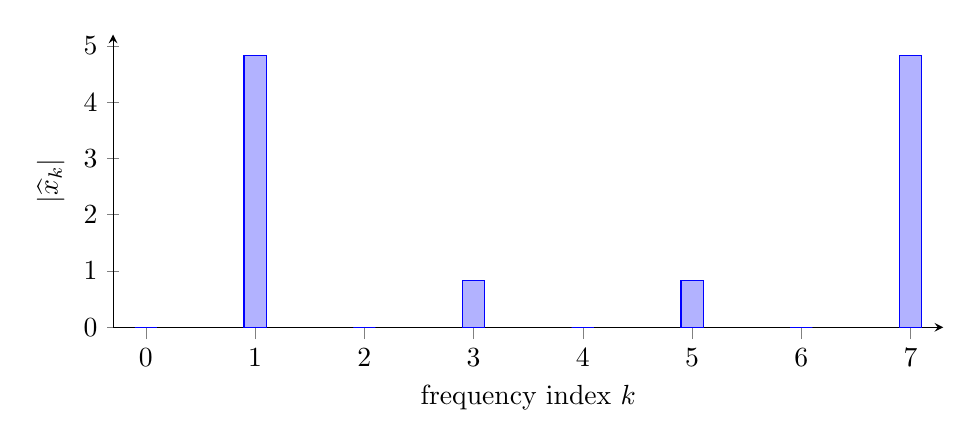
\begin{tikzpicture}
\begin{axis}[
width=\textwidth,
height=5.3cm,
axis lines=left,
xmin=-0.3,xmax=7.3,
ymin=0,ymax=5.2,
xtick={0,1,2,3,4,5,6,7},
ytick={0,1,2,3,4,5},
xlabel={frequency index $k$},
ylabel={$|\widehat{x}_k|$},
ybar,
bar width=8pt,
]
\addplot coordinates {(0,0) (1,4.83) (2,0) (3,0.83) (4,0) (5,0.83) (6,0) (7,4.83)};
\end{axis}
\end{tikzpicture}
\caption{Magnitude of the DFT.}
\end{subfigure}
\caption{The same finite signal viewed in two ways.
In the spatial domain one sees local amplitudes and sign changes.
In the frequency domain one sees which Fourier modes carry most of the energy.
Both descriptions refer to the same object, and convolution may be interpreted in either language.}
\label{fig:spatial-frequency-view}
\end{figure}

\medskip

\Cref{fig:spatial-frequency-view} is pedagogically important.
The left panel displays the signal as a list of local values.
The right panel displays the magnitude of its Fourier coefficients.
Neither picture is more fundamental than the other.
The spatial picture is better for understanding locality and pattern detection.
The spectral picture is better for understanding smoothing, oscillation, and scale selection.
Convolution lives exactly at the interface between them.

\subsection*{Learned filters in spatial and frequency language}

When one says that a convolutional network \emph{learns filters}, there are two equally legitimate interpretations.

\paragraph{Spatial interpretation.}
A learned kernel is a local template.
It may respond to an edge, a corner, a short motif, or a texture.
This is the language in which feature detectors are usually described.

\paragraph{Frequency interpretation.}
The same learned kernel has a frequency response.
It may suppress high-frequency noise, emphasize certain orientations or scales, or selectively pass oscillatory components.
This is the language in which filters are classically described in signal processing.

\medskip

These two descriptions are linked by the convolution theorem.
A kernel that is sharply localized in space often has a broad frequency response,
while a filter highly selective in frequency tends to have more extended spatial support.
This tradeoff is a discrete manifestation of a more general uncertainty principle familiar from harmonic analysis.
Deep learning does not escape that mathematics;
it inherits it.

\medskip

This viewpoint clarifies why the phrase \enquote{learned feature extractor} is not metaphorical.
A convolutional layer literally learns a family of structured linear operators before the nonlinearity is applied.
Those operators are shaped both by local geometry and by frequency selectivity.
The nonlinearity and depth then compose these operators into richer representations,
but the first step already has precise mathematical content.

\subsection*{Multiscale representation and hierarchical processing}

The Fourier viewpoint also helps explain multiscale structure.
Natural signals and images often contain meaningful organization at more than one scale.
Edges and textures are local.
Shapes and object parts are larger.
Global arrangement is larger still.
A useful architecture should therefore not only detect features, but also organize them across scale.

\begin{definition}[Multiscale representation]
A \emph{multiscale representation} of a signal is a family of features that capture structure at different effective spatial or temporal scales.
In layered convolutional models, scale changes arise through repeated local filtering, nonlinear transformation, and downsampling or pooling.
\end{definition}

\medskip

If a single width-$k$ filter sees only a neighborhood of size $k$, then stacked filters and downsampling make progressively larger contexts accessible.
Section 3.2 already formalized this through receptive-field growth.
The Fourier picture adds another interpretation:
coarser layers may be viewed as increasingly selective to larger-scale, slower-varying structure,
while fine-scale layers remain sensitive to local variation.
The resulting hierarchy is one reason convolutional networks work so well on vision tasks.
They do not merely detect local patterns.
They convert local patterns into increasingly global and semantically useful coordinates.

\medskip

This perspective also guards against a common misunderstanding.
It is tempting to say that early layers learn edges and later layers learn objects as if this were an absolute law.
The truth is subtler.
What the network learns depends on the task, the data, and the training objective.
But the architecture does make a general multiscale progression natural:
small-support filters and shallow layers are biased toward local and often higher-frequency structure,
while deeper and coarser layers integrate broader context.

\subsection*{Why this viewpoint matters for deep learning}

The main pedagogical value of the Fourier and multiscale viewpoint is that it prevents convolution from appearing ad hoc.
Convolutional networks are not successful merely because sliding windows happened to work in practice.
They succeed because they instantiate a structured class of linear operators that matches the geometry and scale structure of many natural signals.

\medskip

For mathematics students, this is especially important.
Without the Fourier viewpoint, convolution may look like a useful coding trick.
With it, convolution becomes recognizable as a concrete example of a translation-structured operator,
linked to Toeplitz matrices,
spectral analysis,
filter theory,
and multiscale decomposition.
That is a much deeper and more satisfying picture.

\whattoremember{Convolution has two mathematically linked interpretations.
In the spatial domain it is a local, translation-structured operator.
In the Fourier domain it becomes pointwise multiplication by a frequency response.
This explains smoothing, edge detection, and multiscale processing in one unified language.}

\commonconfusion{The Fourier viewpoint does not replace the spatial viewpoint.
It complements it.
A convolutional kernel is not either a local detector or a frequency filter.
It is both.
The two descriptions are equivalent ways of understanding the same linear operation.}

\subsection*{Exercises}

\begin{exercise}
Let $x \in \mathbb{C}^N$ and let $\delta^{(a)}$ denote the signal that is $1$ at index $a$ and $0$ elsewhere.
Compute $\delta^{(a)} \circledast x$ and explain why this corresponds to circular translation.
How does this connect with translation equivariance?
\end{exercise}

\begin{exercise}
Compute the DFT of the kernel $h=(1,-1)$ for $N=4$ by zero-padding $h$ to length $4$.
At which frequency indices does this filter have the largest magnitude response?
Explain why that matches the intuition that $(1,-1)$ is a difference detector.
\end{exercise}

\begin{exercise}
Let $h_{\mathrm{avg}} = \frac{1}{3}(1,1,1)$.
Show that its frequency response has largest magnitude near zero frequency.
Why does this justify calling it a low-pass filter?
\end{exercise}

\begin{exercise}
A signal is passed through two consecutive convolutions with kernels $w^{(1)}$ and $w^{(2)}$.
Use the convolution theorem to describe the combined frequency response in terms of $\widehat{w^{(1)}}$ and $\widehat{w^{(2)}}$.
How does this help explain the effect of stacking convolutional layers?
\end{exercise}

\begin{exercise}
In practice many neural networks use zero padding rather than circular convolution.
Explain why the discrete convolution theorem is no longer exact in the same form.
Why is the Fourier viewpoint still useful anyway?
\end{exercise}

\subsection*{Notes and references}

The discrete Fourier transform and convolution theorem are standard topics in harmonic analysis and signal processing.
Classical treatments may be found in texts on Fourier analysis, linear systems, and digital signal processing.
Within machine learning, these ideas matter because convolutional networks inherit the mathematics of translation-structured filtering even when presented in modern optimization language.
LeCun and collaborators established the importance of convolutional architectures for vision, while later deep-learning texts such as Goodfellow, Bengio, and Courville gave broad syntheses of their role in representation learning.

\medskip

The multiscale viewpoint connects naturally to wavelets, scale-space methods, and other hierarchical signal representations, although modern convolutional networks are learned rather than hand-designed.
That contrast is one of the main conceptual themes of this chapter:
deep learning keeps the structural assumptions of classical signal processing --- locality, translation structure, multiscale organization --- but learns the filters from data rather than specifying them in advance.
